
\begin{frame} \frametitle{The Population - Greater Melbourne}%
  \vfill %
  Constructing a synthetic agent population, with realistic family household
  structures, that is consistent with person and household level aggregated
  census data distributions.
  
  
  \begin{columns}[T] % align columns
    \begin{column}{.49\textwidth} \begin{itemize} \item Australian Statistical
        Geography Standard (ASGS) specifies 5 granularity levels. \item 
        Statistical
        Area 2 (SA2) is the  $3^{rd}$ smallest \item Greater Melbourne
        \begin{itemize} \item 309 SA2s \item 4,529,496 persons \item 419,693
          households \end{itemize} \end{itemize} \end{column}%
    \hfill%
    \begin{column}{.49\textwidth} \begin{figure} 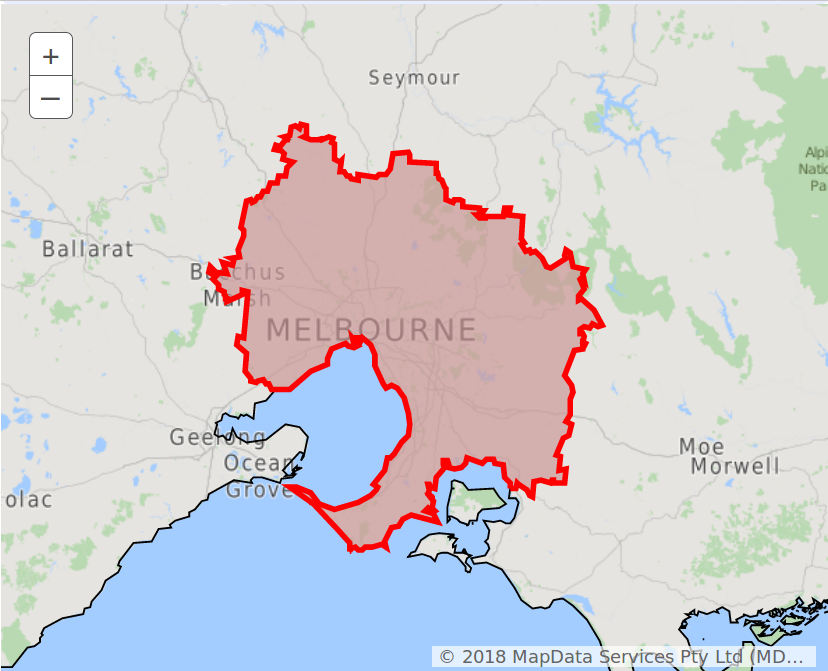
\includegraphics[trim={5cm
          3.5cm 0 3.5cm},clip,scale=0.35] {images/abs-grt-melb} \newline 
          \mbox{\small
          Greater Melbourne Area - www.abs.gov.au} \end{figure} \end{column}%
  \end{columns}%
\end{frame}
  
\begin{frame} \frametitle{Persons Distribution} \begin{center} {\large Number
        of persons by\\ Relationship status $\times$ Sex $\times$ Age range}
    \end{center} \begin{columns}[T] % align columns
    \begin{column}{.3\textwidth} Relationship status \begin{itemize} \item
        Married \item Lone parent \item Dependent under 15 child (U15 Child) 
        \item
        Dependent student (Student) \item Non-dependent over 15 child (O15 
        Child)
        \item Relative \item Group household \item Lone person \end{itemize}
    \end{column}%
    \hfill%
    \begin{column}{.3\textwidth} Sex \begin{itemize} \item Male \item Sex
      \end{itemize} \end{column}%
      \hfill%
      \begin{column}{.3\textwidth} Age range \begin{itemize} \item 0 -- 14
          \item 15 -- 24 \item 25 -- 39 \item 40 -- 54 \item 55 -- 69 \item 70 
          --
          84 \item 85 -- 99 \item 100 or over \end{itemize} \end{column}%
    \end{columns} e.g. \texttt{(married, male, 25 - 39) : 430 persons}\\
    \hspace{2em}\texttt{(student, female, 15 -- 24) : 687 persons}\\
\end{frame}
  
\begin{frame} \frametitle{Relationship status categories} \centering %
    \adjustbox{max height=\dimexpr\textheight-5cm\relax, max
      width=\textwidth}{ \begin{tabular}{|l|l|} %
        \hline %
        \textbf{Custom relationship category} & \textbf{Original ABS
          categories}\\%
        \hline %
        Married&Husband, Wife or Partner in de facto marriage, female same-sex
        couple\\%
        &Husband, Wife or Partner in de facto marriage, male same-sex
        couple\\%
        &Husband, Wife or Partner in de facto marriage, opposite-sex couple\\%
        &Husband, Wife or Partner in a registered marriage\\%
        \hline%
        Lone Parent & Lone parent\\%
        \hline %
        Dependent under 15 child&Foster child under 15\\%
        &Natural or adopted child under 15\\%
        &Otherwise related child under 15\\%
        &Step child under 15\\%
        &Unrelated child under 15\\%
        &Grandchild under15\\%
        \hline%
        Dependent Student& Natural or adopted dependent student\\%
        &Dependent student step child\\%
        &Dependent student foster child\\%
        \hline%
        Non-dependent over 15 child & Non-dependent foster child\\%
        &Non-dependent step child\\%
        &Non-dependent natural, or adopted child\\%
        \hline%
        Relative & Brother/Sister\\%
        &Cousin\\%
        &Father/mother\\%
        &Grandfather/grandmother\\%
        &Nephew/niece\\%
        &Non-dependent grandchild\\%
        &Other related individual (nec)\\%
        &Uncle/aunt\\%
        &Unrelated individual living in family household\\%
        \hline%
        Group household& Group household member\\%
        \hline%
        Lone person & Lone person \\%
        \hline%
        \textit{Ignored}& Visitor(from within Australia)\\%
        &Not applicable\\%
        &Other non-classifiable relationship\\%
        \hline %
      \end{tabular}	%
    } %
\end{frame}
  
\begin{frame} \frametitle{Family households distribution} 
  {
    \small
    \begin{center} { 
        Number of households by\\ Household size $\times$ Family
          household composition} 
    \end{center}
      
    \begin{columns}[T] % align columns
      \begin{column}{.3\textwidth} Household sizes {\small \begin{itemize}
              \item 1 person \item 2 persons \item 3 persons \item ... \item ...
              \item 8 or more persons \end{itemize} } \end{column}%
        \hfill%
        \begin{column}{.6\textwidth}
          
          Family household compositions
          
          \begin{itemize} \item 1 family: Couple family with no children \item
            1 family: Couple family with children \item 1 family: One parent
            family \item 1 family: Other family \item ... \item 3 family: Couple
            family with no children \item 3 family: Couple family with children
            \item 3 family: One parent family \item 3 family: Other family \item
            Group household \item Lone person household
            
          \end{itemize}
          
        \end{column}%
      \end{columns}
      
      e.g. \texttt{(2 persons, 1 family: one parent family) : 30 households}\\
      \hspace{2em}\texttt{(5 persons, 2 family: couple family with children) :
        11 households}\\ }%
\end{frame}
  
\begin{frame}%
  \frametitle{Family Types} %
  \begin{columns}[T]%
    \begin{column}{0.98\textwidth}%
  \begin{itemize}%
    \setlength\itemsep{1em} %
    \item Family composition%
    
    \resizebox{\linewidth}{!}{%
      \begin{tabular}{lll} %
        \small Couple family with no children&\small:&\small Married Male + 
        Married
        Female + 1..* $\times$ Relative\\[2pt]%
        \small Couple family with children&\small :&\small Married Male + 
        Married
        Female + 1..* $\times$ child + 1..* $\times$ Relative\\[2pt]%
        \small Lone parent &\small :&\small Lone parent + 1..* $\times$ child + 
        1..*
        $\times$ Relative\\[2pt]%
        \small Other family&\small :&\small 2..* $\times$ Relative\\[2pt] \small
        Group household&\small :&\small 2..* $\times$ Group household 
        person\\[2pt]%
        \small Lone person household&\small :&\small  Lone person %
      \end{tabular} %
    }%
  \end{itemize}%
\end{column}%
\end{columns}%
\vspace{1em}
  \begin{columns}[T] % align columns
    \begin{column}{.7\textwidth}%
       \begin{itemize}%
        \setlength\itemsep{1em} %
        \item Priority order of deciding the primary family%
        \begin{enumerate}%
          \setlength\itemsep{0.5em}%
          \item The Couple family with children unit in the household %
          \item The One parent family in the household%
          \item Couple with no children and Other families get similar
          priority %
        \end{enumerate} %
        \item     Secondary and tertiary families are not explained in data%
      \end{itemize}%
    \end{column}%
       \begin{column}{.29\textwidth}%
        \begin{figure}
\centering
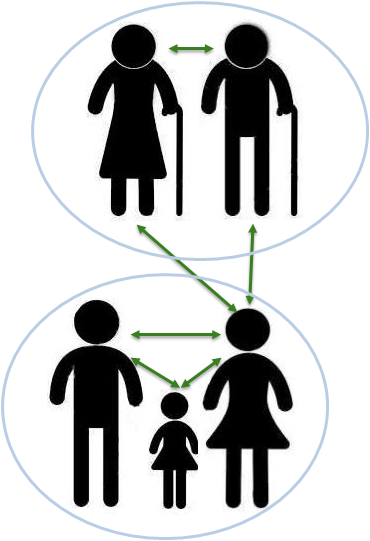
\includegraphics[scale=0.3]{images/family-compo}
\end{figure}

         
        \end{column}%
    \end{columns}%
   
  \end{frame}%
  
  \newcounter{saveenumi}
  \newcommand{\seti}{\setcounter{saveenumi}{\value{enumi}}}
  \newcommand{\conti}{\setcounter{enumi}{\value{saveenumi}}}%
\begin{frame} \frametitle{Data Cleaning} %
	\begin{enumerate}%
		\setlength\itemsep{1em}%
		\item Constructs the population taking household distribution as the 
		reference.%
		\item Set all unrealistic values to 0, e.g. (\texttt{male, married,} 
		\texttt{age
			0-15})	and (\texttt{3 person, lone person household}).%
		\item If the household and person level \texttt{group household} 
		persons are
		different update person level distribution while preserving age and sex
		distribution \item Proportionally update \texttt{lone persons} to match
		\texttt{lone person} households. %
		\item Proportionally update \texttt{married males} and/or 
		\texttt{females} to
		match the number of primary family units consisting married couples%
		
		\seti%
\end{enumerate} \end{frame}
  
\begin{frame} 
  \frametitle{Data Cleaning} 
  \begin{enumerate}
      \setlength\itemsep{1em}%
      \conti %
      \item If the number of \texttt{married males} and \texttt{females} are
      different, no changes are made as this discrepancy is handled by the 
      algorithm.%
      \item If the number of \texttt{lone parents} is less than the
      number of \texttt{one parent} primary family units, increase the
      \texttt{lone parents} proportionally%
      \item If there are not enough \texttt{children} to form all primary
      families that have children increase \texttt{children} categories
      proportionally. %
      \item If the number of \texttt{relatives} is not sufficient to form all 
      primary \texttt{other family} units and \texttt{1 family: couple with no 
      children} {\small (size > 2)} households, increase \texttt{relatives} 
      proportionally.%
      \item If the total number of persons and the number of persons required
      by households are still different, the discrepancy is handled by the
      algorithm.%
  \end{enumerate}%
\end{frame}

\begin{frame}
  \frametitle{Error percentage histograms before and after cleaning}
  
  The error percentage is the difference between the no. of persons in 
  households and the no. of persons in persons distribution as a percentage of 
  the persons in households.
  
  The overall absolute percentage error decreases after cleaning the data.
  \vspace{-1em}
  \begin{figure}%
    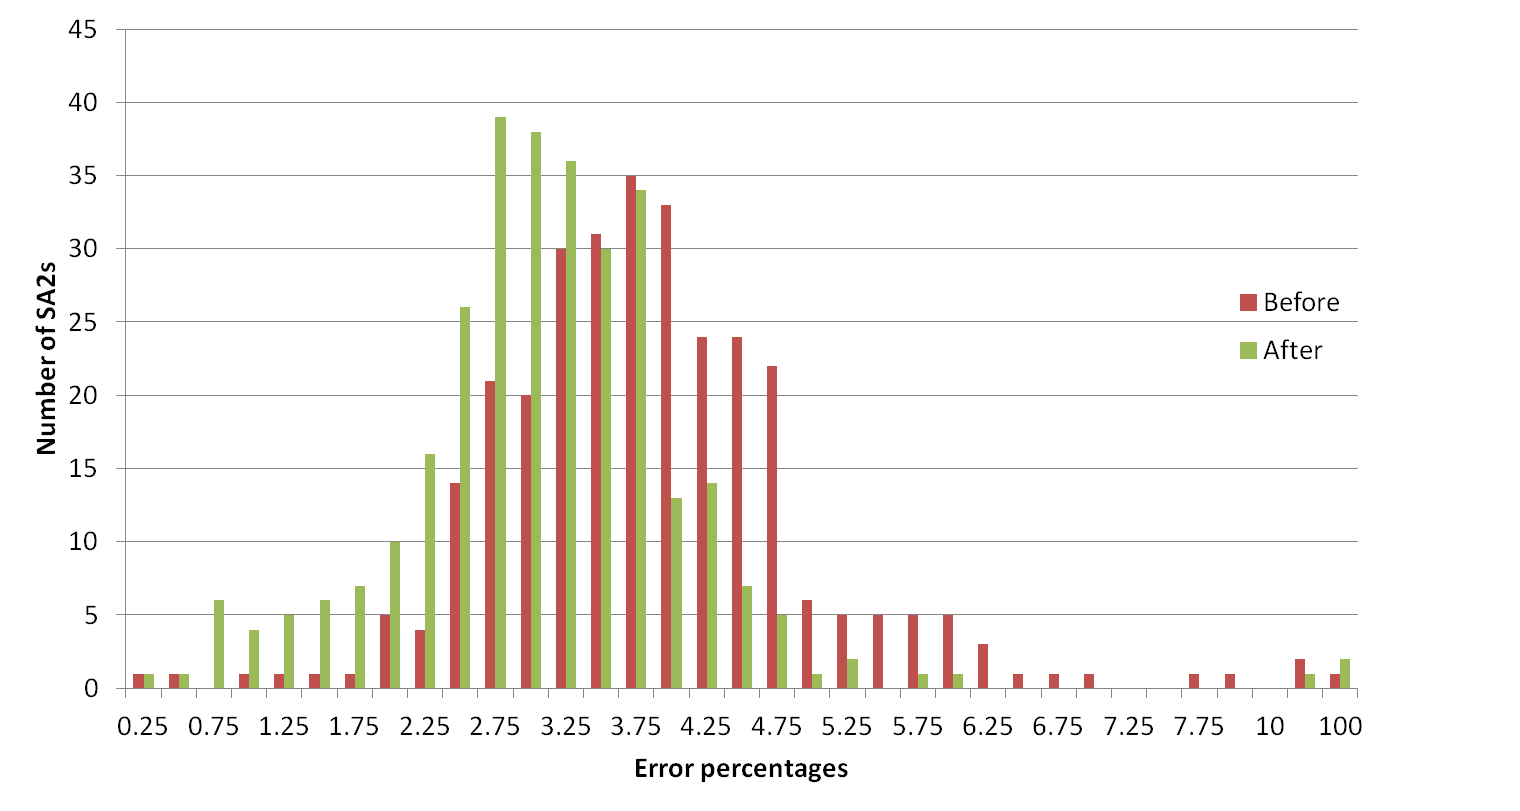
\includegraphics[trim={0.58cm
      0cm 0 1.5cm},clip,scale=0.5] 
    {images/data-cleaning-error}
  \end{figure}%
  
\end{frame}%
    
\begin{frame}%
  \frametitle{Algorithm - Overview}%
  \begin{enumerate}
        \setlength\itemsep{1em}%
        \item Instantiate all the persons with their characteristics. %
        \item Form the basic structures for all the inferable families. %
        \item Instantiate all family households with the primary family, and
        \texttt{group} and \texttt{lone person} households with respective
        person instances.%
        \item Heuristically add non-primary families to the incomplete family
        households.%
        \item Complete households by adding remaining \texttt{children} and
        \texttt{relatives}.%
  \end{enumerate}%
\end{frame}
      
\begin{frame}%
  \frametitle{Algorithm - Instantiate all persons} \begin{enumerate}%
    \setlength\itemsep{1em}%
    \item Instantiate all persons with properties%
    \item If there are extra persons in household level data than person level
    data, create a matching number persons without any characteristics.\\[5pt]%
    \textit{Extras = persons in households distribution - persons in persons
      distribution}%
  	\seti
  \end{enumerate}%
  \begin{figure}
\centering
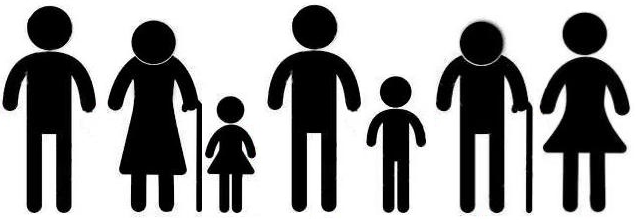
\includegraphics[scale=0.3]{images/form-persons}
\label{fig:form-persons}
\end{figure}

\end{frame}
      
\begin{frame}%
  \frametitle{Algorithm - Form all inferable basic family structures} %
  \begin{enumerate}%
  	\conti %
    \setlength\itemsep{1em}%
    \item Form basic couples by pairing \texttt{married
      males} and \texttt{females} in age descending order.%
    \item Form basic one parent families by pairing each \texttt{lone parent}
    with a \texttt{child} from a younger age category.%
    \item Form the primary \texttt{couple with children} families shown in
    household distribution by pairing a random couple with a \texttt{child} from
    a younger age category.%
    \item Form the primary \texttt{other family} units shown in the household
    distribution by pairing two \texttt{relatives}%
    \seti
  \end{enumerate}%
  \begin{figure}
\centering
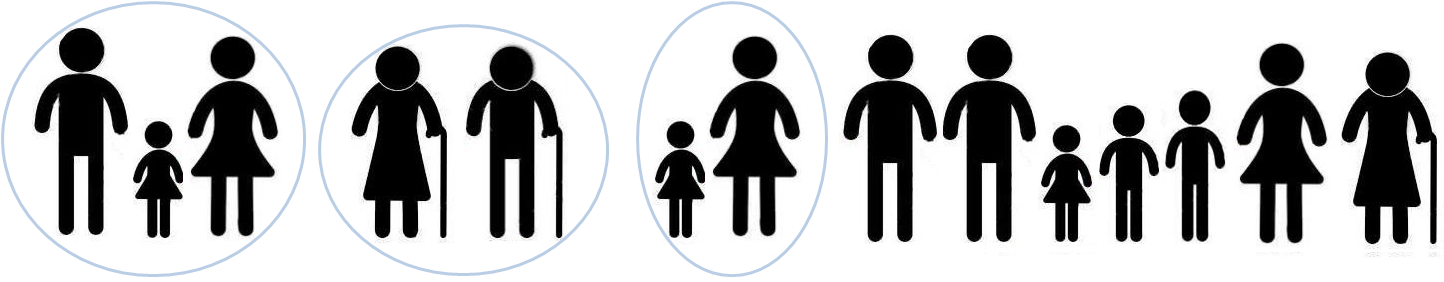
\includegraphics[scale=0.3]{images/form-basic-family}
\end{figure}

\end{frame}%
      
\begin{frame}
  \frametitle{Algorithm - Instantiate all households}
  \begin{enumerate}
  	\conti
    \setlength\itemsep{1em}%
    \item Instantiate empty household instances with the expected properties.%
    \item Add \texttt{lone person} instance to \texttt{lone person} households.%
    \item Add \texttt{group household} person instances to \texttt{group 
    households}.%
    \item Add previously formed basic family units to suitable household 
    instances as primary families, as per households' primary family type 
    descriptions.%
    \seti
  \end{enumerate}%
  \begin{figure}
    \centering
    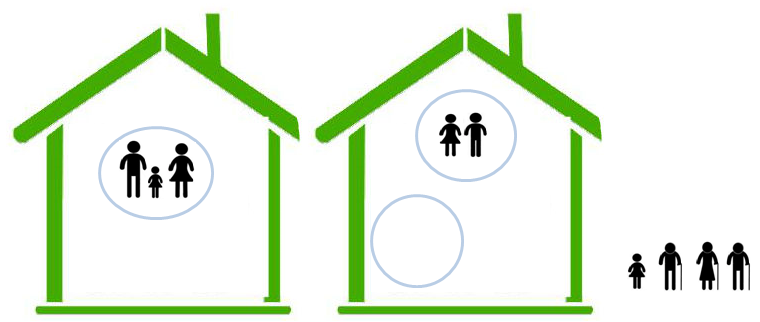
\includegraphics[scale=0.4]{images/form-hhs}
  \end{figure}
\end{frame}%

\begin{frame}%
  \frametitle{Algorithm - Assign non-primary families to households}
  \begin{enumerate}
  	\conti
    \setlength\itemsep{1em}%
    \item Add remaining \texttt{one parent} basic families to eligible 
    households as non-primary families.%
    \item Add remaining \texttt{couples} to households either as a 
    \texttt{couple family with no children} or a \texttt{couple family with 
    children} units.\label{non-prime-cpl-with-child}\\[2pt]%
    \begin{itemize}%
    	\setlength\itemsep{1em}%
    	\item The exact family type is determined based on the probability of
    	observing a non-primary \texttt{couple family with children} unit in a 
    	household.%
    	\item The probability is assumed to be 0.2 (configurable).%
    \end{itemize}%
    \item Add remaining \texttt{lone parents} and \texttt{couples} to the
    \textit{extras} pool by nullifying the relationship category.
    \seti%
  \end{enumerate}%
  \begin{figure}
    \centering
    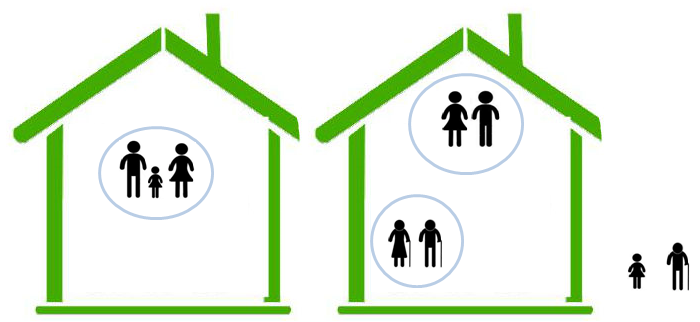
\includegraphics[scale=0.4]{images/add-non-prime}
  \end{figure}
\end{frame}%

\begin{frame}%
	\frametitle{Algorithm - Assign non-primary families to households}%
	\begin{enumerate}%
		\conti%
		\setlength\itemsep{1em}%
		\item Perform next 4 steps if there are households that need more 
		family units.%
		\item Calculate the probability distribution of 
		\texttt{couple}{\small (with and without children)}, 
		\texttt{lone parent} and \texttt{other} family units in primary 
		families.\label{nonprime-dist}%
		\item Determine potential secondary and/or tertiary family types of a 
		household considering heuristic family priority order explained earlier.
		\item Select one of the family types probabilistically based on the 
		distribution calculated in step~\ref{nonprime-dist} and add to the 
		household.%
		\item If the selected family type is \texttt{couple} decide whether to 
		add a \texttt{couple family with no children} or a \texttt{couple 
		family with children} unit as described in 		
		step~\ref{non-prime-cpl-with-child}.%
    \item If certain person types have depleted, use the \textit{extras}.
		\seti%
	\end{enumerate}%
\end{frame}%


\begin{frame}%
  \frametitle{Algorithm - Complete households by adding children and relatives}%
  \begin{enumerate}%
    \setlength\itemsep{1em}%
    \conti%
    \item At this stage all the households have the required family units but
    the number of persons may not be complete.%
    \item Add remaining \texttt{children} to eligible families considering
    parents' ages.%
    \item Add all remaining unassigned person instances, except for
    \texttt{relatives}, to \textit{extras} by nullifying their relationship
    status.%
    \item Probabilistically add all persons in \textit{extras} to families as
    \texttt{children} or \texttt{relatives} based on the input persons
    distribution.%
    \item Add \texttt{relatives} to primary families in remaining incomplete
    households.%
  \end{enumerate}%
  \begin{figure}
    \centering
    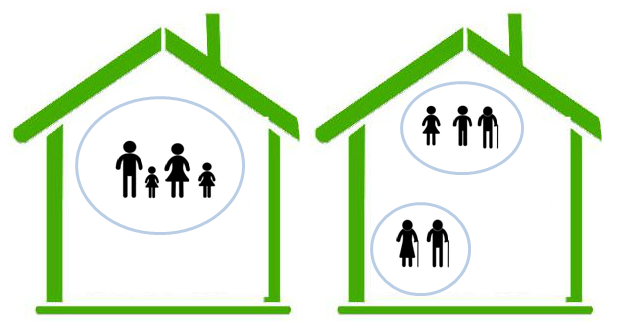
\includegraphics[scale=0.3]{images/add-rels-child}
  \end{figure}
\end{frame}%

\begin{frame}%
	\frametitle{Assigning exact age}%
	
	Assign the exact ages to person instances based on the percentage of 
	persons in each yearly age category in an SA2.\\%
	
	e.g.\\
	
	\begin{itemize}%
		\setlength\itemsep{1em}%
			
		\item Brunswick SA2 synthesised population age distribution\\[2pt]%
		
		\resizebox{0.6\linewidth}{!}{%
			\begin{tabular}{|l|l|l|l|l|l|} %
				\hline%
				\bf Age category&0--14&15--24& .. & 100+\\%
				\hline%
				\bf Persons count&2063&866& .. &0\\%
				\hline%
			\end{tabular} %
		}%
	
		\item Brunswick SA2 exact age distribution\\[2pt]%
		
		\resizebox{0.9\linewidth}{!}{ \begin{tabular}{|l|l|l|l|l|l|l|} %
				\hline%
				\bf Age (year)&0&1&2&3& .. & 115\\%
				\hline%
				\bf Persons percentage&1.12\%&0.98\%&0.87\%&0.86\%&..&0\%\\%
				\hline%
			\end{tabular} %
		}%
	\end{itemize}%
\end{frame}%


\begin{frame}%
	\frametitle{SA1 level household distribution}%
	
	The synthesised households are assigned to SA1s based on the SA1 
	level household types distribution obtained from census data.\\[2pt]%
	\begin{itemize}%
		\setlength\itemsep{1em}%
		\item The households  in synthetic population matches the SA1 level 
		household distribution. %
		\item But the persons distribution may not match the SA1 level 
		persons 
		distribution.%
	\end{itemize}%
\end{frame}%


\begin{frame}%
	\frametitle{Assigning households to addresses}%
	
		
	\begin{enumerate}%
		\setlength\itemsep{1em}%
		\item The address shape files with geographical locations are obtained 
		from Vicmaps (\url{www.data.vic.gov.au}) %
		\item The mesh block polygon shape files are obtained from ABS 
		(\url{www.abs.gov.au})%
		\item Find the ABS mesh block and the SA1 of each address using GIS tools.
    \item Assign synthesised households in an SA1 to corresponding addresses.
	\end{enumerate}%
\end{frame}%

\begin{frame}
  \frametitle{Cosine similarity test results preprocessed census data vs. 
  synthesised}
  
  \begin{figure}%
    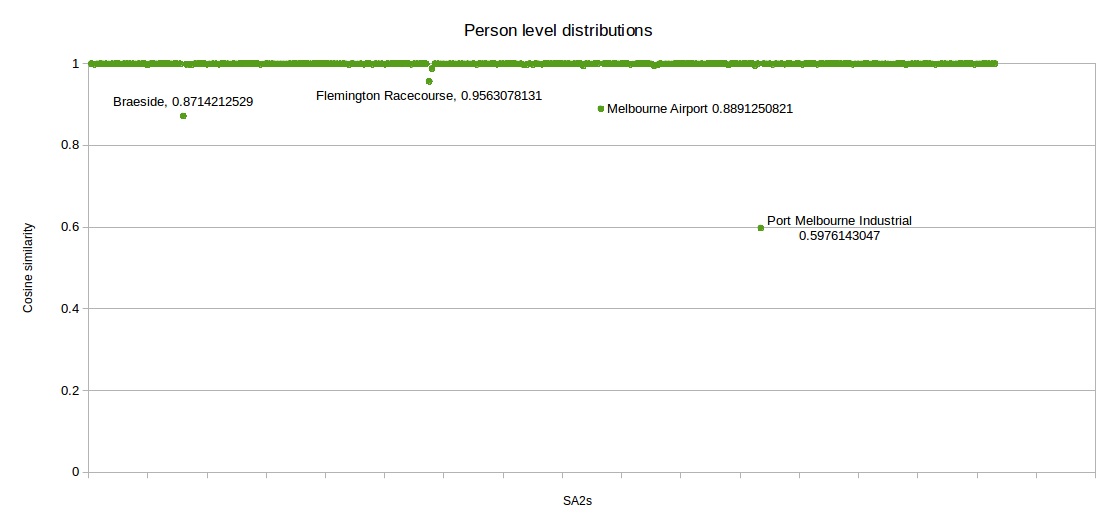
\includegraphics[trim={0.5cm
      0 0 0},clip,scale=0.55] 
      {images/cosine-similarity-preprocessed-vs-synth}
  \end{figure}%
  
\end{frame}%

\begin{frame}
  \frametitle{Cosine similarity test results raw census data vs. synthesised}
  
  \begin{figure}%
    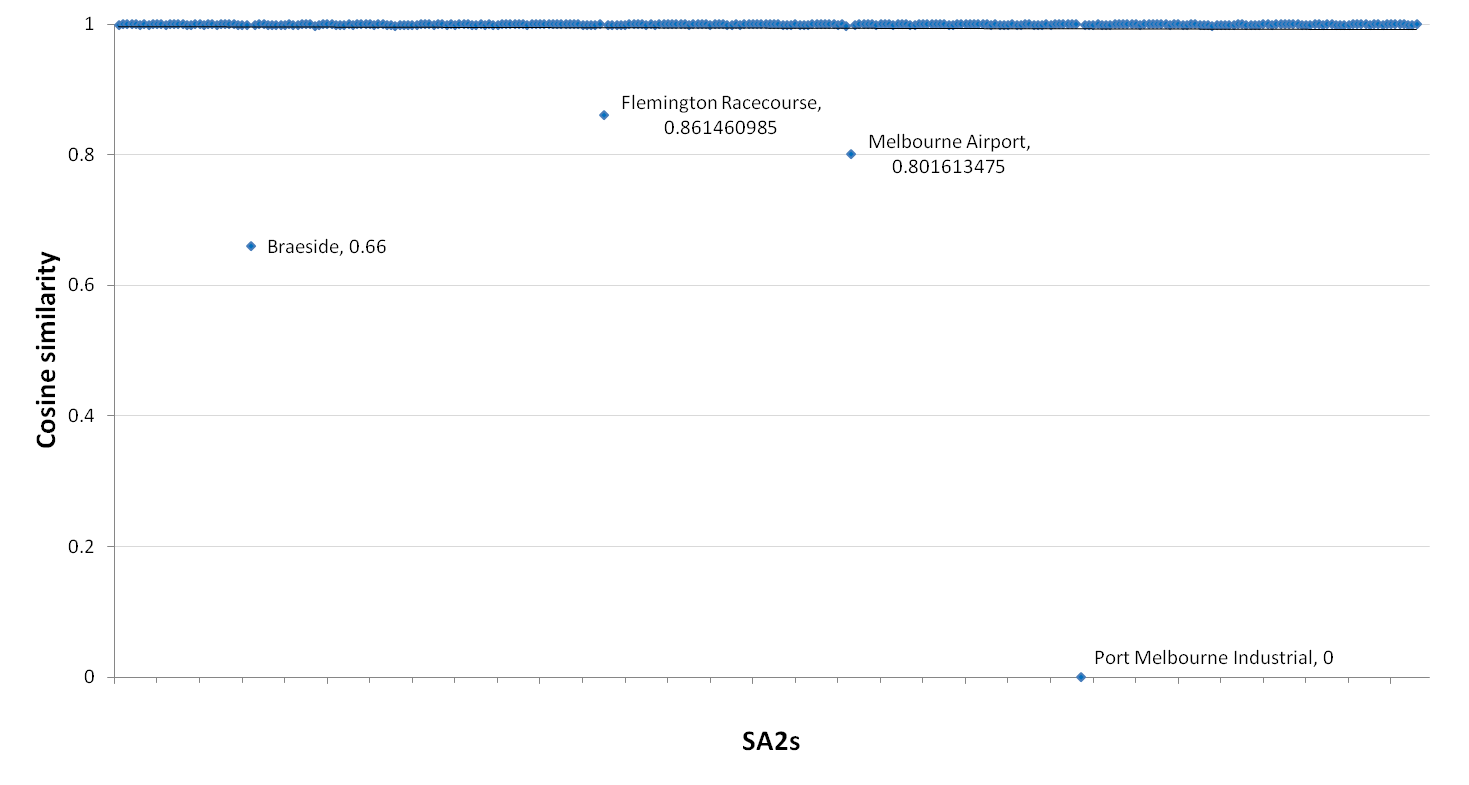
\includegraphics[trim={0.5cm
      0 0 0},clip,scale=0.52] 
    {images/cosine-similarity-raw-vs-synth}
  \end{figure}%
  
\end{frame}%

\begin{frame}
  \frametitle{Melbourne SA2  persons distribution - synthesised vs. 
  preprocessed 
  census data}
  \begin{itemize}
    \item Total persons:32,046
    \item Wrongly categorised persons: 52
  \end{itemize}
  \vspace{-3em}
  \begin{figure}%
    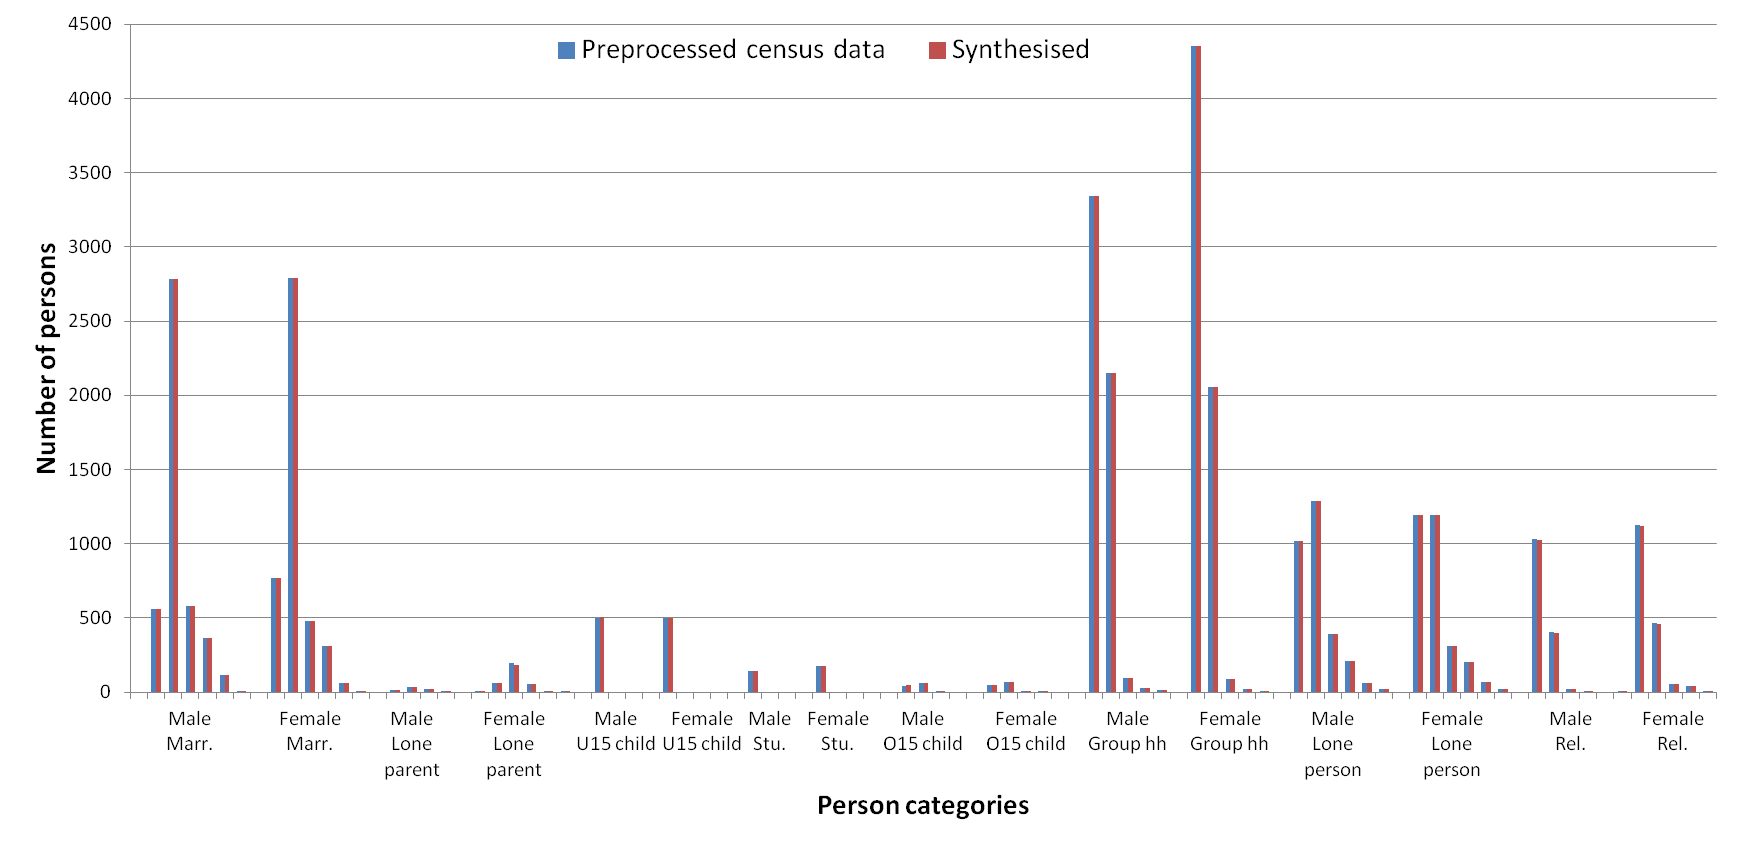
\includegraphics[trim={0.58cm
      0 0 0},clip,scale=0.43] 
    {images/good-melb-person-bar}
  \end{figure}%
  
\end{frame}%

\begin{frame}
  \frametitle{Person types distribution - Melbourne Airport SA2}
  \begin{itemize}
    \item Persons in input person level data: 63
\item Persons in synthetic population: 32
\item Absolute error: 31
\item Persons in input household distribution: 32
  \end{itemize}
    \vspace{-2em}
  \begin{figure}%
    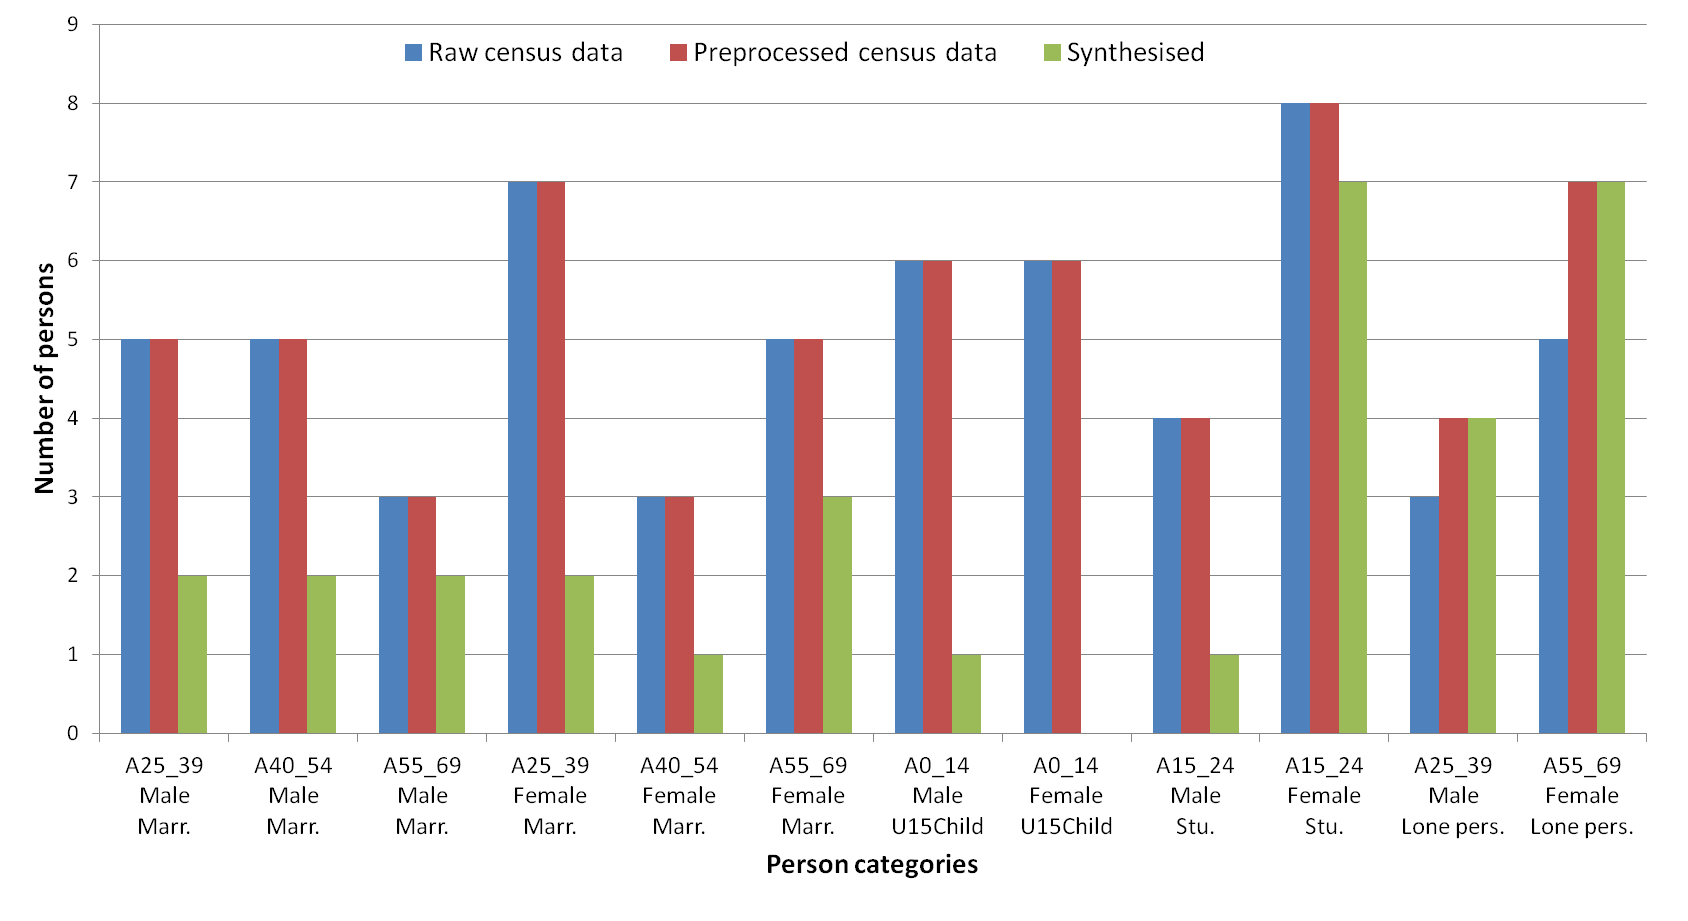
\includegraphics[trim={0.5cm
      0 0 0},clip,scale=0.45] {images/melb-airport-person-bar}
  \end{figure}%
  
\end{frame}%

\begin{frame}
  \frametitle{Household types distribution - Melbourne Airport SA2}
    All households are formed though significant person level discrepancies are 
    observed%
    \begin{itemize}
      \item Total households: 17
    \end{itemize}
\vspace{-2em}
\begin{figure}%
  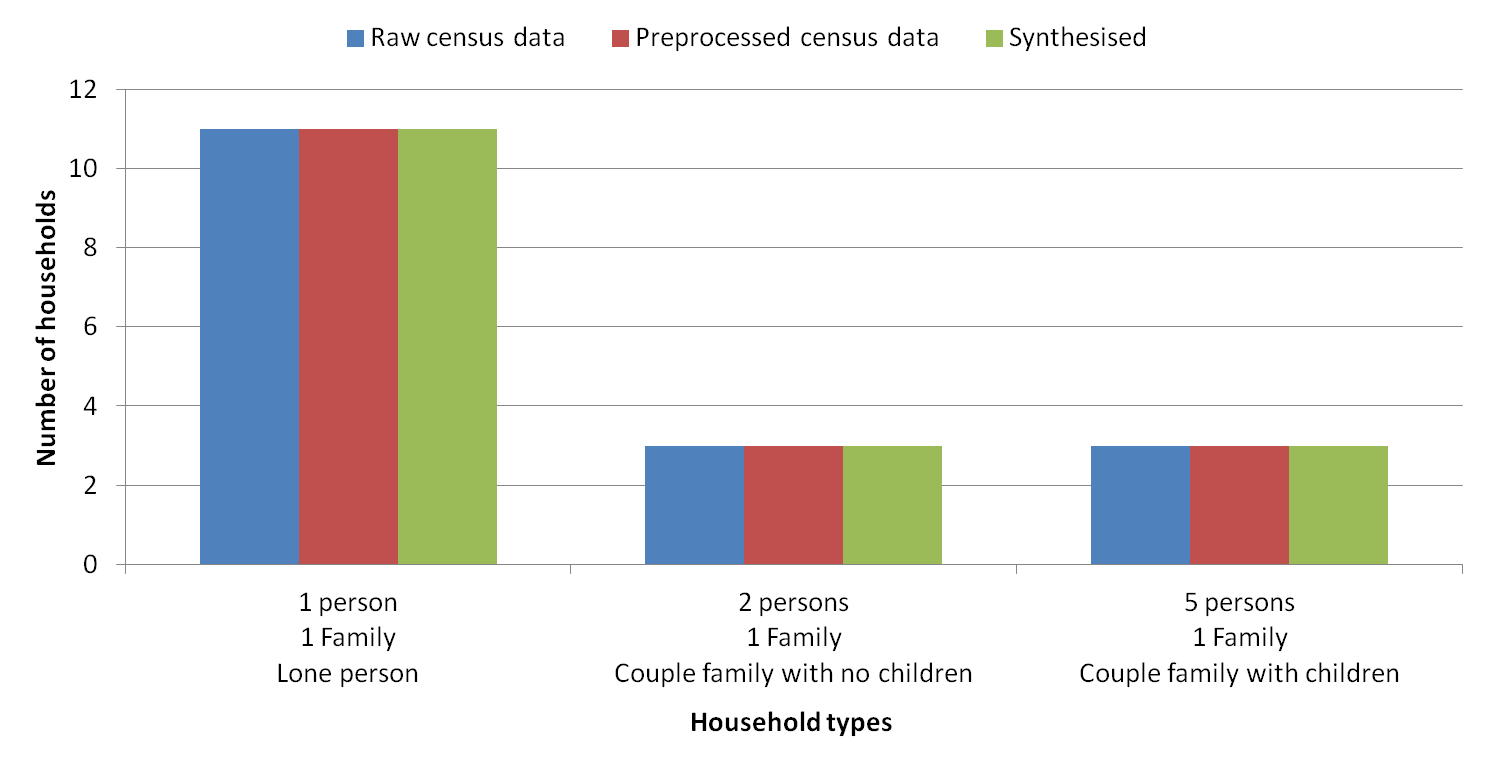
\includegraphics[trim={0.5cm
    0 0 0},clip,scale=0.5] {images/melb-airport-hh-bar} \newline
\end{figure}%

\end{frame}%

\begin{frame}
  \frametitle{ }
\begin{center}
{\huge \bf \textcolor{rmitred}{Thank you and Questions?}}\\
\vspace{4em}
  Source code\\ \url{www.github.com/agentsoz/synthetic-population}
\end{center}
  
  

  
  
\end{frame}%






